\documentclass[12pt,a4paper,onecolumn]{article}%twocolumn
\usepackage[top=2.5cm,bottom=2.0cm,left=2.0cm,right=2.0cm]{geometry}
\usepackage{bm,dcolumn,amsmath,graphicx,amsfonts,amssymb,fancyhdr}

\usepackage{hyperref}
\usepackage{xcolor}
\definecolor{cite}{rgb}{0.,0.,0.95}   % more subtle than the default blue
\hypersetup{colorlinks,	linkcolor={cite}, citecolor={cite},	urlcolor={cite}}


% Some handy commands:
\renewcommand{\v}[1]{\ensuremath{\boldsymbol{#1}}}	%bold-math for vectors
\newcommand{\braket}[1]{\ensuremath{\langle #1\rangle}}	%Dirac BraKets
\newcommand{\bra}[1]{\ensuremath{\langle #1|}}	%Dirac Bras
\newcommand{\ket}[1]{\ensuremath{|#1\rangle}}	%Dirac Kets

% Define C++ syntax highlighting colour scheme
\usepackage{listings}
\lstdefinelanguage{cpp}{
  language=C++,
  basicstyle=\footnotesize\ttfamily,
  numbers=left,
  numberstyle=\scriptsize,
  tabsize=2,
  breaklines=true,
  escapeinside={@}{@},
  numberstyle=\tiny\color{lightgray},
  keywordstyle=\color{violet},
  stringstyle=\color{olive}\ttfamily,
  identifierstyle=\color{blue},%violet
  commentstyle=\color{gray},
  emphstyle=\color{red},
  frame=single,
  rulecolor=\color{lightgray},
  rulesepcolor=\color{lightgray},
  showstringspaces=false,
  morekeywords={constexpr}, 
}
\lstset{language=cpp}

%=================================================
\pagestyle{fancy}
\fancyhead[L]{Title}
\fancyhead[R]{Tristan Burns/42648493 -- \today}

%Make section headers smaller:
\usepackage[tiny]{titlesec}

%=================================================
\begin{document}


%=================================================
\section{Introduction}


%=================================================
\section{B1}

\textit{1.}
\begin{align*}
\langle nlm|r|n'l'm' \rangle &= \int \psi_{nlm}^\dag(\mathbf{r})r\psi_{n^\prime l^\prime m^\prime} (\mathbf{r}) r^2 sin\theta dr d\theta d\phi\\
\langle nlm|r|n'l'm' \rangle &= \int \frac{P^*_{nl}(r)}{r} r \frac{P_{n'l'}(r)}{r} r^2 dr \int_0^\pi \int_0^{2\pi} Y_{lm}^*(\theta, \phi) Y_{l'm'}(\theta, \phi) \sin \theta d\theta d\phi\\
\langle nlm|r|n'l'm' \rangle &= \int P^*_{nl}(r) r P_{n'l'}(r)  dr  \left(\delta_{ll^\prime}  \delta_{mm^\prime}\right)\\
\langle nlm|r|n'l'm' \rangle &= \int P^*_{nl}(r) r P_{n'l'}(r) dr   \\
\end{align*}

Where we make use of the of the orthagonal spherical components.

Thus, the problem reduces to solving the radial equation (6), which depends on the potential V ,

\textit{2}
%=================================================
\section{...}

You can see my plot in Fig.~\ref{fig:my-plot}.

\begin{figure}[h!]
\centering
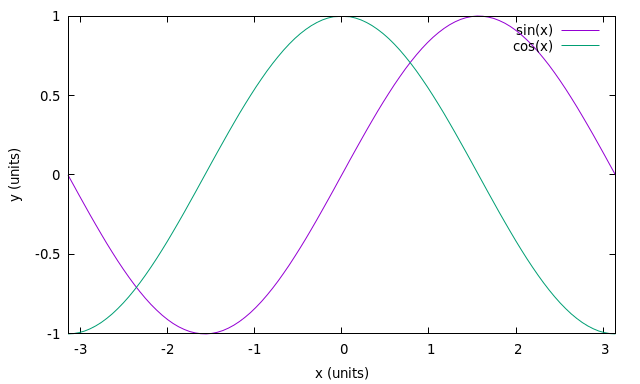
\includegraphics[width=0.5\textwidth]{Template-plot.png}
\caption{\label{fig:my-plot}Caption for the plot}
\end{figure}


%=================================================
\section{B5}

You can add code snippets like this:

\begin{lstlisting}
double f(double x) {
    std::cout << "Hello world\n";
    return std::exp(-x) * std::sin(5.0 * x);
}
\end{lstlisting}

%=================================================
\section{Conclusion}

\end{document}






